\documentclass{article}
\usepackage[utf8]{inputenc}
\usepackage{amsmath, amssymb}
\usepackage{mathtools}
\usepackage{tikz}
\usepackage{pgfplots}
\usetikzlibrary{positioning}

\title{DSBA Calculus HW6}
\author{Kirill Korolev, 203-1}
\date{14th of October, 2020}

\begin{document}
	
\maketitle

\begin{enumerate}
\item Give formal definition for the following notions. Construct the negation to each of them:

\begin{align*}
&\lim_{x \to a-0} f(x) = L\\
&\forall \epsilon > 0, \exists \delta > 0 : \forall x \in D(f) \quad a - \delta < x < a \quad |f(x) - L| < \epsilon\\
&\exists \epsilon > 0: \forall \delta > 0, \exists x \in D(f) \quad a - \delta < x < a \quad |f(x) - L| \geq \epsilon\\\\
&\lim_{x \to -\infty} f(x) = +\infty\\
&\forall \epsilon > 0, \exists \delta > 0 : \forall x \in D(f) \quad x < -\frac{1}{\delta} \quad f(x) > \frac{1}{\epsilon}\\
&\exists \epsilon > 0: \forall \delta > 0, \exists x \in D(f) \quad x < -\frac{1}{\delta} \quad f(x) \leq \frac{1}{\epsilon}
\end{align*}

\item Find the following one-sided limits:

\begin{align*}
\lim_{x \to 7+0} \frac{|x-7|}{x^2+5x-14} = \lim_{x \to 7+0} \frac{x-7}{(x-7)(x+2)} = \lim_{x \to 7+0} \frac{1}{x+2} = \frac{1}{9}\\
\lim_{x \to 7-0} \frac{|x-7|}{x^2+5x-14} = \lim_{x \to 7-0} -\frac{x-7}{(x-7)(x+2)} = \lim_{x \to 7-0}-\frac{1}{x+2} = -\frac{1}{9}
\end{align*}

\item Find the following one-sided limits:
\begin{align*}
&\lim_{x \to -1+0} \frac{\sin{x} + 1}{x + 1}\\
&\sin{x} + 1 \geq 0 \quad \forall x \in \mathbb{R}\\
&x + 1 \geq 0 \quad x \to -1+0  \Rightarrow
\lim_{x \to -1+0} \frac{\sin{x} + 1}{x + 1} = +\infty\\
&\lim_{x \to -1-0} \frac{\sin{x} + 1}{x + 1}\\
&x + 1 \leq 0 \quad x \to -1-0  \Rightarrow
\lim_{x \to -1+0} \frac{\sin{x} + 1}{x + 1} = -\infty
\end{align*}

\item Sketch the graph of the piecewise defined function and find limits:

\begin{align*}
f(x)=
\begin{cases}
2\sin{(x+1)}, \quad x \leq -1\\
3 - x^2 - 2x, \quad x > -1
\end{cases}
\end{align*}

\begin{tikzpicture}
\begin{axis}
\addplot[smooth,samples=200,domain=-10:-1]{2*sin(deg(x+1))};
\addplot[smooth,samples=200,domain=-1:2]{3 - x^2 - 2*x};
\end{axis}
\end{tikzpicture}

\begin{align*}
\lim_{x \to -1-0} f(x) = \lim_{x \to -1-0} 2\sin{(x+1)} = 0\\
\lim_{x \to -1+0} f(x) = \lim_{x \to -1+0} 3 - x^2 - 2x = 4\\
\end{align*}

$\lim_{x \to -1} f(x)$ doesn't exist because left and right one-sided limits are not equal.
\newpage
\item Find $a_i$ and $b_i$ such that:

\begin{align*}
&\lim_{x \to +\infty} (\sqrt{x^2-x+1} - a_1 x - b_1) = 0\\
&\lim_{x \to +\infty} (\frac{x^2-x+1 - a_1^2 x^2 - 2a_1b_1x - b_1^2}{\sqrt{x^2-x+1} + a_1 x + b_1}) = 0\\
&\lim_{x \to +\infty} (\frac{(1-a_1^2)x^2 - (1 + 2a_1b_1)x + 1 - b_1^2}{\sqrt{x^2-x+1} + a_1 x + b_1}) = 0\\
&\lim_{x \to +\infty} (\frac{(1-a_1^2)x - (1 + 2a_1b_1) + \frac{1 - b_1^2}{x}}{\sqrt{1-\frac{1}{x}+\frac{1}{x^2}} + a_1 + \frac{b_1}{x}}) = 0\\
&1-a_1^2 = 0 \Rightarrow a_1 = \pm \sqrt{1} \quad \text{But} \: \sqrt{x^2-x+1} \to \infty, \quad x \to \infty \Rightarrow\\
&a_1 = 1 \Rightarrow \lim_{x \to +\infty} (\frac{(1-a_1^2)x - (1 + 2a_1b_1) + \frac{1 - b_1^2}{x}}{\sqrt{1-\frac{1}{x}+\frac{1}{x^2}} + a_1 + \frac{b_1}{x}}) = \lim_{x \to +\infty} \frac{-1 - 2b_1}{2} = 0\\
&b_1 = -\frac{1}{2}
\end{align*}

For limit when $x \to -\infty$ the same considerations hold with exception that $\sqrt{x^2-x+1} \to -\infty, \quad x \to -\infty \Rightarrow a_1 = -1$, therefore $1 - 2b_1 = 0 \Rightarrow b_1 = \frac{1}{2}$

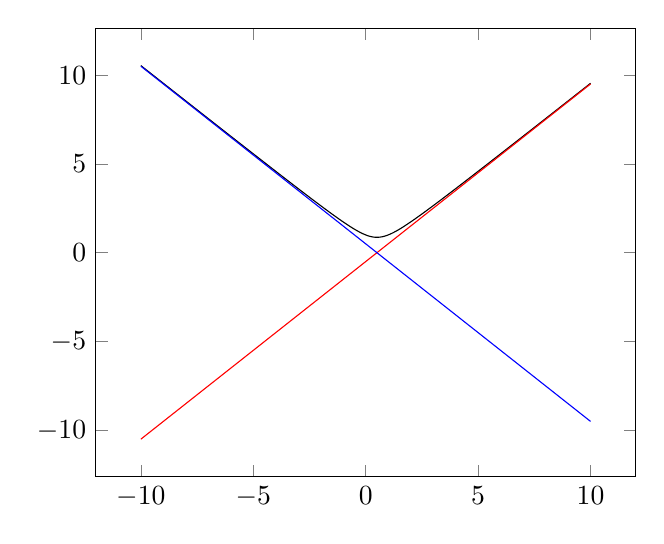
\begin{tikzpicture}
\begin{axis}	
\addplot[smooth,samples=200,domain=-10:10]{sqrt(x^2-x+1)};
\addplot[smooth,color=red,samples=200,domain=-10:10]{x - 0.5};
\addplot[smooth,color=blue,samples=200,domain=-10:10]{-x + 0.5};
\end{axis}
\end{tikzpicture}

\newpage
\item Evaluate the following limits:

\begin{align*}
&\lim_{x \to 0} \frac{\tan{5x}}{\sin{2x}} = \lim_{x \to 0} \frac{2x\sin{(5x)}5x}{2x\cos{(5x)}\sin{(2x)}5x} =
\lim_{x \to 0} \frac{5x}{2x} = \frac{5}{2} 
\end{align*}

\begin{align*}
&\lim_{x \to \frac{\pi}{2}} \cos{x} \cdot \sin{\frac{2}{2x - \pi}}\\
&\cos{\frac{\pi}{2}} = 0 \quad -1 \leq \sin{\frac{2}{2x - \pi}} \leq 1 \Rightarrow \lim_{x \to \frac{\pi}{2}} \cos{x} \cdot \sin{\frac{2}{2x - \pi}} = 0
\end{align*}

\begin{align*}
&\lim_{x \to 0} \frac{1 - \cos{8x}}{5x^2} = \lim_{x \to 0} \frac{2\sin^2{4x}}{5x^2} = \lim_{x \to 0} \frac{2\sin^2{(4x)}16x^2}{5x^216x^2} = \frac{32}{5}
\end{align*}

\begin{align*}
\lim_{x \to 0} \frac{2x-5x^2+x^3}{\sin{3x}} = \lim_{x \to 0} \frac{3x(2-5x+x^2)}{3\sin{3x}} = \lim_{x \to 0} \frac{2-5x+x^2}{3} = \frac{2}{3}
\end{align*}

\begin{align*}
\lim_{x \to 0} x \cdot \cot{(5x)} = \lim_{x \to 0} x \frac{\cos{5x}}{\sin{5x}} = \lim_{x \to 0} 5x \frac{\cos{5x}}{5\sin{5x}} = \frac{1}{5}
\end{align*}

\end{enumerate}

\end{document}